\mode*

% Since this a solution template for a generic talk, very little can
% be said about how it should be structured. However, the talk length
% of between 15min and 45min and the theme suggest that you stick to
% the following rules:  

% - Exactly two or three sections (other than the summary).
% - At *most* three subsections per section.
% - Talk about 30s to 2min per frame. So there should be between about
%   15 and 30 frames, all told.


\section{Multi-Lateral Security}

%\begin{frame}{\insertsubsectionhead}
%  \begin{quote}
%    Privacy is a transient notion.
%    It started when people stopped believing that God could see everything and 
%    stopped when governments realised there was a vacancy to be filled.
%  \end{quote}
%  \begin{flushright}
%    Roger Needham
%  \end{flushright}
%\end{frame}

\subsection{The Lattice model}

\begin{frame}
  \begin{idea}
    \begin{itemize}
      \item The less people that know a secret, the better.
      \item \enquote{Need-to-know basis}: the principle of least priviledge.
    \end{itemize}
  \end{idea}
\end{frame}

\begin{frame}{\insertsubsectionhead}
  \begin{figure}
    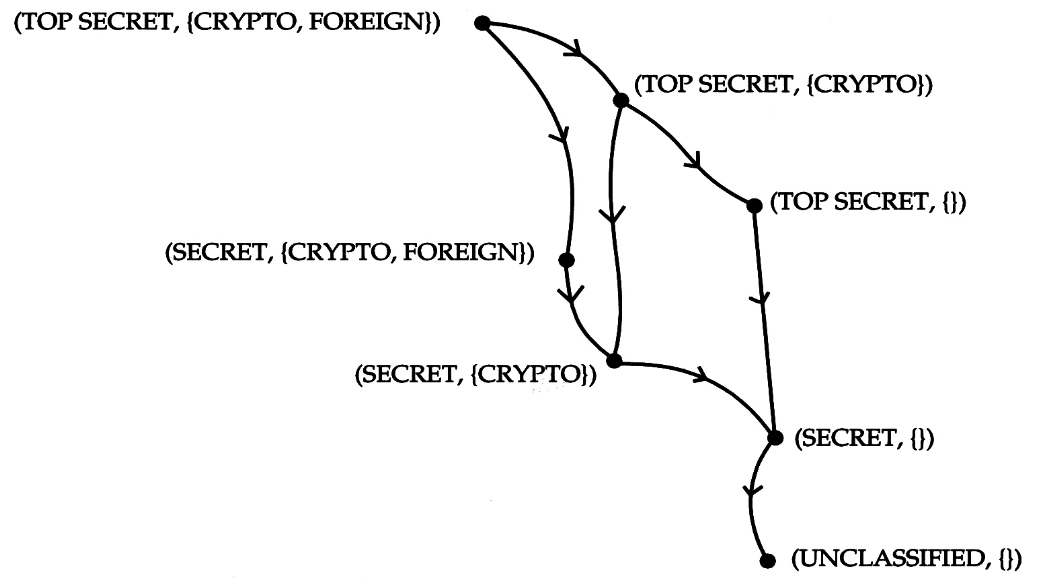
\includegraphics[height=0.6\textheight]{lattice.png}
    \caption{The Lattice Model, turns BLP from an ordered set into a partially 
      ordered set.}
  \end{figure}
\end{frame}

\begin{frame}
  \begin{definition}[Multilateral security]
    \begin{itemize}
      \item We add code words to classifications.
      \item A classification together with code words is a \emph{compartment}.
      \item This is \emph{multilateral security}.
    \end{itemize}
  \end{definition}
\end{frame}

\subsection{The Chinese Wall Model}
\begin{frame}
  \begin{idea}
    \begin{itemize}
      \item Developed by Brewer och Nash.
      \item Origin: banks.
      \item \emph{Separation of duty}:
        A user may do \(A\) or \(B\), but not both.
    \end{itemize}
  \end{idea}
\end{frame}

\begin{frame}
  \begin{definition}[The Chinese Wall Model]
    \begin{itemize}
      \item Resource~\(c\).
      \item Owner~\(y(c)\) of \(c\).
      \item Classification~\(x(c)\) of \(c\), conflict of interest class.
    \end{itemize}

    \begin{description}
      \item[Simple security property]
        Subject~\(s\) can access \(c\)
        if and only if
        for all \(c'\) that \(s\) can read from, either
        \(y(c)\notin x(c')\) or \(y(c) = y(c')\).

      \item[*-property] Subject~\(s\) can write to \(c\)
        if and only if
        \(s\) cannot read any \(c'\) such that \(x(c')\neq \emptyset\) and 
        \(y(c)\neq y(c')\).
    \end{description}
  \end{definition}
\end{frame}

%\subsection{BMA-modellen}
%\begin{frame}[allowframebreaks]{\insertsubsectionhead}
%  \begin{itemize}
%    \item Varje patientjournal har en åtkomstkontrollista (\emph{access control 
%        list}, ACL) med alla som får läsa och skriva till journalen.
%    \item För att komma åt journal:
%      \begin{itemize}
%        \item En läkare får öppna journalen med sig själv och patienten på 
%          ACL:en.
%        \item Vid remiss, en läkare får öppna journalen med sig själv, 
%          patienten och remitterande läkare på ACL:en.
%      \end{itemize}
%    \item Ägare: en läkare är ansvarig och kontrollerar ACL.
%    \item Notifiering: alla förändringar av ACL notifieras till och godkänns av 
%      patienten.
%    \item Beständighet: ingen kan ta bort data inom en förutbestämd tidsperiod.
%    \item Loggning: all åtkomst till journalen noteras i den med subjektets 
%      identitet, tid och datum.
%    \item Informationsflöde: information från journal \(A\) får föras över till 
%      journal \(B\) om och endast om \(B\):s ACL är en del av \(A\):s.
%    \item Sammanställningskontroll: patienter ska få en särskild notifiering om 
%      någon person med tillgång till en stor mängd patientjournaler föreslås 
%      läggas till ACL:en.
%    \item Trusted computing base: datorsystem som hanterar patientjournaler ska 
%      påtvinga dessa principer.
%  \end{itemize}
%\end{frame}

%\subsection{Inference control}
%
%\begin{frame}{\insertsubsectionhead}
%  \begin{itemize}
%    \item Att avanonymisera statistik: Vad är medelbetyget för alla kvinnliga 
%      studenter på Nätverksdriftsprogrammet i åk 1?
%    \item Om det inte går: Vad är medelbetyget för alla studenter på 
%      Nätverksdriftsprogrammet, och vad är medelbetyget för alla manliga 
%      studenter på Nätverksdriftsprogrammet?
%      \begin{itemize}
%        \item Nu kan jag beräkna medelbetyget för våra kvinnliga deltagare.
%      \end{itemize}
%  \end{itemize}
%\end{frame}

\subsection{A final example}

\begin{frame}
  \begin{figure}
    \includegraphics[width=\textwidth]{qubes.png}
  \end{figure}
  \url{https://qubes-os.org}
\end{frame}


%%% REFERENCES %%%

\begin{frame}[allowframebreaks]
  \printbibliography
\end{frame}
